\graphicspath{{5coset/asy/}}
\setcounter{section}{4}

\section{Cosets \& Factor Groups --- HOMEWORK EXS!}\label{chap:coset}

The overarching goal of this chapter is to partition a group into subsets in such a way that the \emph{set of subsets} inherits a natural group structure. This is a long and abstract story, though it is really nothing new; it is precisely the idea behind modular arithmetic!

\begin{example}{}{cosetsimple}
	In $\Z_3=\{0,1,2\}$ the elements are really \emph{subsets} $[0],[1],[2]$ of the \emph{integers} $\Z$: that is,
	\begin{gather*}
		[0]=\{x\in\Z:x \equiv 0\negthickspace\pmod 3\} =\{\ldots,-3,0,3,6,\ldots\}\\
		[1]=\{x\in\Z:x \equiv 1\negthickspace\pmod 3\} =\{\ldots,-2,1,4,7,\ldots\}\\
		[2]=\{x\in\Z:x \equiv 2\negthickspace\pmod 3\} =\{\ldots,-1,2,5,8,\ldots\}
	\end{gather*}
	When we write $1\operatorname{\textcolor{blue}{+_3}}2=0\in\Z_3$, what we really mean is
	\[
		\forall x\in[1], y\in[2]
		\text{ we have }
		x\operatorname{\textcolor{red}{+}}y\in [0]
	\]
	The \textcolor{red}{group operation (addition)} on $\Z$ naturally induces the \textcolor{blue}{group operation (addition modulo 3)} on the set of subsets $\Z_3=\{[0],[1],[2]\}$. 
\end{example}


\subsection{Cosets \& Normal Subgroups}\label{sec:cosetnormal}

Our primary goal is to generalize Example \ref{ex:cosetsimple}. Start by observing that the identity element $[0]\in\Z_3$ is a \emph{subgroup} of $\Z$ from which the other subsets $[1]$, $[2]$ may be obtained by \emph{translation.}

\begin{defn}{}{}
	Let $H$ be a subgroup of $G$ and $g\in G$. The \emph{left coset} of $H$ containing $g$ is 
	\[
		gH:=\{gh:h\in H\}\tag{$x\in gH\iff \exists h\in H$ such that $x=gh$}
	\]
	This is a subset of $G$. The \emph{right coset} of $H$ containing $g$ is defined similarly:
	\[
		Hg:=\{hg:h\in H\}
	\]
	The \emph{identity coset} $H=eH=He$ is the left \& right coset of $H$ containing the identity $e$.\smallbreak
	$H$ is a \emph{normal subgroup} of $G$, written $H\triangleleft G$, if the left and right cosets containing $g$ are always equal
	\[
		H\triangleleft G
		\iff
		\forall g\in G,\ gH=Hg
	\]
\end{defn}

If $G$ is written additively, then the left and right cosets of $H$ containing $g$ are instead written
\[
	g+H:=\{g+h:h\in H\}
	\qquad\qquad 
	H+g:=\{h+g:h\in H\}
\]

\begin{example*}{\ref{ex:cosetsimple} cont}{}
	Let $G=\Z$ and $H=[0]=3\Z$. The left and right cosets of $H$ are precisely the elements of $\Z_3$:
	\begin{gather*}
		3\Z=0+3\Z=3\Z+0=[0]=\{\ldots,-3,0,3,6,\ldots\}\\
		1+3\Z=3\Z+1=[1]=\{\ldots,-2,1,4,7,\ldots\}\\
		2+3\Z=3\Z+2=[2]=\{\ldots,-1,2,5,8,\ldots\}
	\end{gather*}
	Since the left and right cosets are equal, $H=3\Z$ is a normal subgroup of $\Z$.
\end{example*}

\goodbreak

The last observation is in fact general---the proof is an exercise.

\begin{lemm}{}{cosetbasic1}
	Every subgroup of an abelian group $G$ is normal.
\end{lemm}


A subgroup of a non-abelian group \emph{might} be normal, but is more likely not to be (see Example \ref*{ex:cosetexs}.\ref{ex:nonnormalcosets}).


\begin{examples}{}{cosetexs}
	\exstart\label{ex:cosets1} The subgroup $H=\ip 2=\{0,2,4\}\le\Z_6$ has two distinct cosets (left $=$ right since $\Z_6$ is abelian):
	\begin{align*}
		H&=\{0,2,4\}&&\bigl(=2+H=4+H\bigr)\\
		1+H&=\{1,3,5\}&&\bigl(=3+H=5+H\bigr)
	\end{align*}
	Observe how the cosets \textbf{partition} $\Z_6$ into equal-sized subsets.
	
% 	\exstart\label{ex:cosets1} Consider the subgroup $H=\ip 4=\{0,4,8\}\le\Z_{12}$. This is cyclic with order 3. The distinct cosets of $\ip 4$ are as follows (left $=$ right since $\Z_{12}$ is abelian!):
% 	\begin{align*}
% 		\ip 4 &=\{0,4,8\}&&\bigl(=4+\ip 4=8+\ip 4\bigr) \hspace{220pt}\\
% 		1+\ip 4 &=\{1,5,9\}&&\bigl(=5+\ip 4=9+\ip 4\bigr)\\
% 		2+\ip 4 &=\{2,6,10\}&&\bigl(=6+\ip 4=10+\ip 4\bigr)\\
% 		3+\ip 4 &=\{3,7,11\}&&\bigl(=7+\ip 4=11+\ip 4\bigr)
% 	\end{align*}
% 	Observe how the cosets \emph{partition} $\Z_{12}$ into equal-sized subsets. 

	\begin{enumerate}\setcounter{enumi}{1}
		\item\label{ex:nonnormalcosets} The left and right cosets of the subgroup $H=\{e,\mu_1\}\le D_3$ are as follows:
		\[
			\renewcommand{\arraystretch}{1.15}
			\begin{array}{l@{\hspace*{.3cm}}|@{\hspace*{.3cm}}l}
		  	\text{Left cosets} & \text{Right cosets}\\\hline
				H=\mu_1H=\{e,\mu_1\}& H=H\mu_1=\{e,\mu_1\}\\
				\rho_1H=\mu_3H=\{\rho_1,\mu_3\} & H\rho_1=H\mu_2=\{\rho_1,\mu_2\}\\
				\rho_2H=\mu_2H=\{\rho_2,\mu_2\} & H\rho_2=H\mu_3=\{\rho_1,\mu_3\}
			\end{array}
		\]
		To verify this, either revisit the multiplication table for $D_3$ (Example \ref{ex:d3}) or use cycle notation (e.g. Example \ref{ex:disym}).	This time the left and right cosets of $H$ are not the same: $H$ is \emph{not} a normal subgroup of $D_3$. The \textbf{partitioning} observation still holds: the left cosets partition $D_3$ into three equal-sized subsets; the right cosets also partition $D_3$ into equal-sized (but different) subsets.
	
	  
		\begin{minipage}[t]{0.65\linewidth}\vspace{0pt}
			\item\label{ex:cosetsubspace} Consider a 1-dimensional subspace $\textcolor{blue}{W}\le\R^2$. Each coset
			\[
				\textcolor{Green}{\vu+W} =\{\vu+\vw:\vw\in W\}
			\]
			is a line parallel to $W$. Once again, the cosets (all lines parallel to $W$) \textbf{partition} $\R^2$.\smallbreak
			If this feels too abstract, consider the special case where $W$ is the $y$-axis: each coset is a vertical line (same $x$-co-ordinate).\smallbreak
			More generally, if $W$ is a subspace of some vector space, then the cosets $\vu+W$ are the sets parallel to $W$. Only the zero coset $W=\V0+W$ is a sub\emph{space.}
		\end{minipage}
		\hfill
		\begin{minipage}[t]{0.33\linewidth}\vspace{0pt}
			\flushright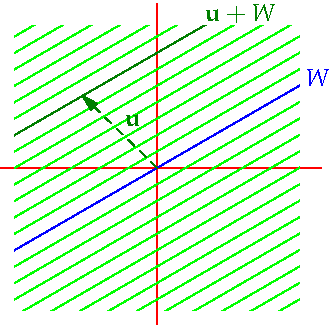
\includegraphics[scale=0.93]{coset-coset}
		\end{minipage}
	
	
		\item Consider the alternating group $A_n$ as a subgroup of $S_n$. Generalizing the argument from Theorem \ref{thm:alt}, we see that for any $\alpha\in A_n$ and $\sigma\in S_n$,
		\[
			\alpha\sigma\text{ even }
			\iff \sigma\text{ even }
			\iff \sigma\alpha\text{ even}
		\]
		Otherwise said, for any $\sigma\in S_n$ the cosets of $A_n$ containing $\sigma$ are
		\[
			\sigma A_n=A_n\sigma=
			\begin{cases}
				A_n&\text{if $\sigma$ even}\\
				B_n&\text{if $\sigma$ odd}
			\end{cases}
		\]
		where $B_n$ is the set of odd permutations in $S_n$. In particular, $A_n$ is a normal subgroup of $S_n$.
	\end{enumerate}
\end{examples}


\goodbreak


As observed in the examples, the cosets of any subgroup $H\le G$ partition $G$.

\begin{thm}{}{cosetpart}
	Let $H$ be a subgroup of $G$. Then the left cosets of $H$ partition $G$. Moreover,
	\[
		y\in xH
		\mathrel{\textcolor{blue}{\iff}} x^{-1}y\in H
		\mathrel{\textcolor{red}{\iff}} xH=yH
	\]
	The right cosets also partition $G$:
	\[
		y\in Hx\iff yx^{-1}\in H\iff Hx=Hy
	\]
\end{thm}

The \textcolor{blue}{blue} criterion is often very easy to check. Before reading the proof, convince yourself that each of our previous examples satisfies the result. When $H$ is non-normal, the right cosets partition $G$ differently to the left cosets (e.g.\ Example \ref*{ex:cosetexs}.\ref{ex:nonnormalcosets}).

\begin{example}{}{}
	This should seem familiar when $G=\Z$ and $H=n\Z$. Written additively,
	\[
		a+H=b+H\mathrel{\textcolor{red}{\iff}} b-a\in H\iff n\mid b-a \iff a\equiv b\pmod n
	\]
	The cosets of $H$ are precisely the equivalence classes modulo $n$. Indeed you've likely encountered the main proof in the context of modular arithmetic.
\end{example}

\begin{proof}
	We start by verifying the \textcolor{blue}{first connective}.
	\[
		y\in xH
		\iff \exists h\in H\text{ such that }y=xh
		\iff x^{-1}y=h\in H
	\]
	Now define a relation $\sim$ on $G$ via $x\sim y\Longleftrightarrow x^{-1}y\in H$. We claim that this is an equivalence relation:
	\begin{quote}
		\begin{description}\itemsep2pt
			\item[\normalfont\emph{Reflexivity}:] $x\sim x$ since $x^{-1}x=\textcolor{Green}{e\in H}$.
			\item[\normalfont\emph{Symmetry}:] $x\sim y\Longrightarrow x^{-1}y\in H \mathrel{\textcolor{Green}{\Longrightarrow}} y^{-1}x=(x^{-1}y)^{-1}\in H \Longrightarrow y\sim x$.
			\item[\normalfont\emph{Transitivity}:] If $x\sim y$ and $y\sim z$ then $x^{-1}y\in H$ and $y^{-1}z\in H$. But \textcolor{Green}{$H$ is closed}, whence
			\[
				x^{-1}z=(x^{-1}y)(y^{-1}z)\in H\implies x\sim z
			\]
		\end{description}
	\end{quote}
	The equivalence classes therefore partition $G$. Since $x\sim y\iff y\in xH$, the equivalence class of $x$ is indeed the left coset $xH$.\qedhere
\end{proof}



The \textcolor{Green}{subgroup status} of $H$ is precisely what guarantees a partition (compare Theorem \ref{thm:subgroup}):
\begin{quote}
	\begin{description}\itemsep2pt
		\item[\normalfont\emph{Reflexivity}:]  $H$ contains the \textcolor{Green}{identity} (and is thus \textcolor{Green}{non-empty}).
		\item[\normalfont\emph{Symmetry}:] $H$ satisfies the \textcolor{Green}{inverse axiom}.
		\item[\normalfont\emph{Transitivity}:] $H$ is \textcolor{Green}{closed} under the group operation.
	\end{description}
\end{quote}

When $H$ is not a subgroup, the coset construction need not produce a partition.

\begin{example}{}{}
	The \emph{subset} $H=\{0,1\}\subseteq\Z_3$ is not a subgroup. Its left `cosets' fail to partition $\Z_3$:
	\[
		H=\{0,1\},\quad 1+H=\{1,2\},\quad 2+H=\{2,1\}
	\]
\end{example}


\goodbreak

By combining the criteria in Theorem \ref{thm:cosetpart}, we obtain a useful result for identifying when a subgroup is normal \emph{without} explicitly having to compute its cosets. The proof is an exercise.

\begin{cor}{}{normalconj}
	Normal subgroups are precisely those which are closed under \textbf{conjugation}:
  \[
  	H\triangleleft G\iff H\le G\text{ and \ }\forall g\in G,\ \forall h\in H, \	gh g^{-1}\in H
  \]
\end{cor}

Since this holds for all $g$, we may equivalently observe $g^{-1}hg\in H$. 

% \begin{proof}
% 	Start by using the criteria in Theorem \ref{thm:cosetpart} to observe:
% 	\begin{enumeratea}
% 	  \item $gH\subseteq Hg\iff \forall h\in H,\ gh\in Hg \iff \forall h\in H,\ gh g^{-1}\in H$
% 	  \item $Hg\subseteq gH\iff \forall h\in H,\ hg\in gH \iff \forall h\in H,\ g^{-1}hg\in H$
% 	\end{enumeratea}
% 	We now complete the proof in two parts:
% 	\begin{description}
% 		\item[\normalfont $(\Rightarrow)$] $H\triangleleft G$ means $\forall g\in G,\ Hg=gH$, and so implies part (a) for all $g\in G$. 
% 		\item[\normalfont $(\Leftarrow)$] If $gh g^{-1}\in H$ for all $g,h$, then this is also true for $g^{-1}$: that is $g^{-1}hg\in H$. We now have the right side of both (a) and (b). Otherwise said, $gH=Hg$ for all $g\in G$, whence $H$ is normal in $G$.\qedhere
% 	\end{description}
% \end{proof}


\goodbreak


\begin{exercises}{}{}
	Key concepts:\quad \emph{left/right cosets \& partitioning\quad normal subgroup\quad kernels are normal}

	\begin{enumerate}
	  \item Find the cosets of each subgroup: since the groups are abelian, left and right cosets are equal.
		\begin{enumerate}
	  	\item $2\Z\le\Z$\qquad\quad
	  	(b) $4\Z\le 2\Z$\qquad\quad
		  (c) $\ip{4}\le\Z_{10}$\qquad\quad
		  (d) $\ip{6}\le\Z_{30}$\qquad\quad
		  (e) $\ip{20}\le\Z_{30}$
		\end{enumerate}
			
			
		\item\label{exs:VfactorV} Find the cosets of $H=\bigl\{(0,0),(2,0),(0,2),(2,2)\bigr\}\le\Z_4\times\Z_4$
			
			
		\item Find the left and right cosets of $\{\rho_0,\rho_1,\rho_2\}\le D_3$. Is the subgroup normal?
		
		
		\item\label{exs:va4}\begin{enumerate}
		  \item Find the left and right cosets of $H:=\{e,(1\,2\,3),(1\,3\,2)\}\le A_4$. Is the subgroup normal?
		  \item Repeat the question for the subgroup $V:=\{e,(1\,2)(3\,4),(1\,3)(2\,4),(1\,4)(2\,3)\}$
		\end{enumerate}
		
	
		\item\label{exs:d4normal}\begin{enumerate}
		  \item Find the left and right cosets of $H=\{\rho_0,\delta_1\}\le D_4$. Is $H$ normal? (see Examples \ref{ex:disym})
			\item Repeat for the subgroup $K=\{\rho_0,\rho_2\}$.
		\end{enumerate}
		(\emph{Hint: Use cycle notation as in Example \ref{ex:disym}})
	  
	  
	  \item Prove Lemma \ref{lemm:cosetbasic1}: every subgroup of an abelian group is normal.
	  
	  
	  \item\label{exs:partitioncoset} Suppose $H$ is a \emph{subset} of $G$, but not necessarily a subgroup.
	  \begin{enumerate}
	    \item If $H$ has only one element, show that the sets $gH=\{gh:h\in H\}$ do partition $G$.
	    \item Show that the `cosets' of $H=\{1,3\}$ also partition $\Z_4$, even though $H$ is not a subgroup.
	  \end{enumerate}
	  
	
		\item Let $H=\{\sigma\in S_4:\sigma(4)=4\}$. Show that $H$ is a subgroup of $S_4$. Is it \emph{normal}?
		
		
		\item Prove Corollary \ref{cor:normalconj}.
	  
	  
	  \item\label{exs:directprodfactor}\begin{enumerate}
	    \item Suppose $G=H\times K$, \ $J\triangleleft H$ and let $\widetilde J=J\times\{e_K\}$. Prove that $\widetilde J\triangleleft G$.\par
	    (\emph{When $J=H$ this is often written $H\triangleleft (H\times K)$. A similar result holds for $K$.})
	    \item Explain how Example \ref*{ex:cosetexs}.\ref{ex:cosetsubspace} fits into part (a).
	  \end{enumerate} 
	  
		
		\item Let $H,K$ be subgroups of $G$. Define $\sim$ on $G$ by
		\[
			a\sim b\iff \exists h\in H,\ k\in K \ \text{ such that }\ a=hb k
		\]
		\begin{enumerate}
	  	\item Prove that $\sim$ is an equivalence relation on $G$ and describe the elements of the equivalence class of $a\in G$; this is called a \emph{double coset}.
	  	\item Compute the double cosets of $H=\{e,(1\,2)\}$ and $K=\{e,(1\,3)\}$ as subgroups of $S_3$. 
		\end{enumerate}

	\end{enumerate}
\end{exercises}


\clearpage


\subsection{Lagrange's Theorem \& Indices}\label{sec:lagrange}


We've been inching towards a powerful result; hopefully you've hypothesized this already!

\begin{thm}{Lagrange}{lagrange}
	In a finite group, the order of a subgroup divides the order of the group:\footnotemark
	\[
		H\le G\implies \nm H\Big\vert \nm G
	\]
\end{thm}

Note that the converse is \emph{false}: e.g.{} $A_4$ has order 12, but no subgroup of order 6 (Exercise \ref*{sec:transpositions}.\ref{exs:a4subgroups}). The argument is merely a generalized version of the proof of Theorem \ref{thm:alt} ($\nm{A_n}=\frac 12\nm{S_n}$).

\footnotetext{%
	This is often misremembered as `the order of an element divides the order of the group,' which is the special case when $H$ is a \emph{cyclic subgroup} of $G$. Corollary \ref{cor:subscyclic} is the even more special case when $G$ is cyclic:
	$\ip s\le\Z_n$ has order $\frac n{\gcd(s,n)}$.
}


\begin{proof}
	Suppose $H\le G$ and fix $g\in G$. The function \emph{left-multiplication by $g$}
	\[
		L_g:H\to gH:h\mapsto gh
	\]
	is a bijection (with inverse $L_g^{-1}:gh\mapsto h$). Every left coset of $H$ therefore has the same cardinality as $H$. Since the left cosets partition $G$ (Theorem \ref{thm:cosetpart}), we conclude that
	\[
		\nm G=\text{(number of left cosets of $H$)}\cdot \nm H
		\implies \nm H\Big\vert \nm G
		\tag*{\qedhere}
	\]
\end{proof}


We could instead have proved Lagrange via the right coset partition. Here is an example of its power.

\begin{cor}{}{}
	Up to isomorphism, there is a unique group of prime order $p$, namely $\Z_p$.
\end{cor}

\begin{proof}
	Suppose $G$ is a group with prime order $p$. Since $p\ge 2$, we may choose some element $g\neq e$. The order of the cyclic subgroup $\ip{g}\le G$ satisfies:
	\begin{itemize}%\itemsep0pt
	  \item $\nm{\ip g}\ge 2$ since $g\neq e$.
	  \item $\nm{\ip{g}}=1$ or $p$ by Lagrange, since $p$ is prime.
	\end{itemize}
	We conclude that $\nm{\ip g}=p\implies G=\ip{g}$ is cyclic and thus isomorphic to $\Z_p$ (Theorem \ref{thm:cyclicisomorph}).
\end{proof}

\begin{example}{}{}
	$G=\Z_4\times\Z_2$ has order 8 so its non-trivial proper subgroups can only have orders 2 or 4 and are thus isomorphic to $\Z_2$, $\Z_4$ or $\textcolor{blue}{V}$. These can be identified by thinking about all possible generators; $V$ requires three elements of order 2 which we indeed have! Here is the subgroup diagram: all proper subgroups are cyclic except \textcolor{blue}{$V=\{(0,0),(2,0),(0,1),(2,1)\}$}.
	\[
		\def\arraystretch{1.1}
		\begin{array}[t]{@{}c|c|c}
			\text{generator}&\text{order}&\text{subgroup}\\\hline
			(1,0)\text{ or }(3,0) & 4 & \{(0,0),(1,0),(2,0),(3,0)\}\\
			(1,1)\text{ or }(3,1) & 4 & \{(0,0),(1,1),(2,0),(3,1)\}\\
			(2,0) & 2 & \{(0,0),(2,0)\}\\
			(0,1) & 2 & \{(0,0),(0,1)\}\\
			(2,1) & 2 & \{(0,0),(2,1)\}\\
			(0,0) & 1 & \{(0,0)\}
		\end{array}
		\qquad
		\xymatrix @R13pt{%
			&\Z_4\times\Z_2 \ar@/_0pc/@{-}[dl] \ar@{-}[d] \ar@{-}[dr]&\\
			\ip{(1,0)} \ar@{-}[dr] & \textcolor{blue}{V} \ar@{-}[dl] \ar@{-}[d] \ar@{-}[dr] & \ip{(1,1)} \ar@{-}[dl]\\
			\ip{(0,1)} \ar@{-}[dr] & \ip{(2,0)} \ar@{-}[d] & \ip{(2,1)} \ar@{-}[dl] &\\
			&\ip{(0,0)}&
		}
	\]
\end{example}


\goodbreak


The proof of Lagrange tells us that the \emph{number} of left and right cosets of $H\le G$ is \emph{identical:} both equal the quotient $\frac{\nm G}{\nm H}$. This motivates a new concept.

\begin{defn}{}{index}
	The \emph{index} $(G:H)$ of a subgroup $H\le G$ is the cardinality of the set of (left) cosets:
	\[
		(G:H)=\nm{\{gH:g\in G\}}
	\]
\end{defn}

The index is also the cardinality of the set of \emph{right} cosets (Exercise \ref{exs:indexcard}). If $G$ is finite, then $(G:H)=\frac{\nm G}{\nm H}$.


\begin{examples}{}{indexeasy}
	\exstart If $G=\Z_{20}$ and $H=\ip{2}$, then there are $(G:H)=\frac{20}{10}=\frac{\nm G}{\nm H}=2$ cosets:
	\[
		H=\ip{2}=\{0,2,4,\ldots,18\}
		\quad\text{and}\quad 
		1+H=\{1,3,5,\ldots,19\}
		\]
	\begin{enumerate}\setcounter{enumi}{1}
	  \item\label{ex:indexeasy2} Recall (Example \ref{ex:orthogonal} \& Exercise \ref*{sec:subgroup}.\ref{exs:subgpmatrix}) the orthogonal and special orthogonal groups
	  \[
	  	\rO_n(\R)=\{A\in M_n(\R):A^TA=I\},\qquad
	  	\rSO_n(\R)=\{A\in\rO_n(\R):\det A=1\}
	  \]
	  Since every orthogonal matrix has determinant $\pm 1$, it feels as if $\rSO_n(\R)$ should be `half' of $\rO_2(\R)$. Since both groups are infinite (indeed uncountable), we need the index to confirm this intuition. Recall Theorem \ref{thm:cosetpart}: given $A,B\in\rO_n(\R)$,
	  \[
	  	A\,\rSO_n=B\,\rSO_n(\R)
	  	\iff B^{-1}A\in\rSO_n(\R)
	  	\iff \det(B^{-1}A)=1
	  	\iff \det B=\det A
	  \]
	  We conclude that there are precisely two cosets $\bigl(\rO_n(\R):\rSO_n(\R)\bigr)=2$.
	\end{enumerate}
\end{examples}


\begin{thm}{}{tower}
	If $K\le H\le G$ is a sequence of subgroups, then
	\[
		(G:K)=(G:H)(H:K)
	\]
\end{thm}

If $G$ is a finite group then the result is essentially trivial:
\[
	(G:K)=\frac{\nm G}{\nm K}
	=\frac{\nm G}{\nm H}\cdot\frac{\nm H}{\nm K}
	=(G:H)(H:K)
\]
Our proof also covers infinite groups and infinite indices. You are \emph{strongly} encouraged to work through the following examples, which are written in the language of the proof.



\begin{proof}
	Choose an element $\textcolor{red}{g_i}$ from each left coset of $H$ in $G$ and an element $\textcolor{blue}{h_j}$ from each left coset of $K$ in $H$. Plainly
	\[
		(G:H)=\nm{\{\textcolor{red}{g_i}\}}
		\qquad\text{and}\qquad 
		(H:K)=\nm{\{\textcolor{blue}{h_j}\}}
	\]
	We claim that the left cosets of $K$ in $G$ are precisely the sets $(\textcolor{red}{g_i}\textcolor{blue}{h_j})K$. Certainly each such is a \emph{coset}; we show that these cosets \emph{partition} $G$, whence the collection $\{(\textcolor{red}{g_i}\textcolor{blue}{h_j})K\}$ must comprise \emph{all} left cosets.
	\begin{itemize}
	  \item Every $g\in G$ lies in some left coset of $H$, so $\exists \textcolor{red}{g_i}\in G$ such that $g\in \textcolor{red}{g_i}H$.\par
	  $\textcolor{red}{g_i}^{-1}g\in H$ lies in some left coset of $K$ in $H$, so $\exists \textcolor{blue}{h_j}\in H$ such that $\textcolor{red}{g_i}^{-1}g\in \textcolor{blue}{h_j}K$.\par
	  But then $g\in (\textcolor{red}{g_i}\textcolor{blue}{h_j})K$ so that every $g\in G$ lies in at least one set $(\textcolor{red}{g_i}\textcolor{blue}{h_j})K$.
	  \item Suppose $y\in \textcolor{red}{g_i}\textcolor{blue}{h_j}K\cap \textcolor{red}{g_\alpha} \textcolor{blue}{h_\beta}K$. Since $K\le H$ and the left cosets of $H$ partition $G$, we have
	  \[
	  	y\in \textcolor{red}{g_i}H\cap \textcolor{red}{g_\alpha} H
	  	\implies \textcolor{red}{g_\alpha}=\textcolor{red}{g_i}
	  \]
	  But then $\textcolor{red}{g_i}^{-1}y\in \textcolor{blue}{h_j}K\cap \textcolor{blue}{h_\beta} K\implies \textcolor{blue}{h_\beta}=\textcolor{blue}{h_j}$ similarly, since the left cosets of $K$ in $H$ partition $H$. It follows that the sets $(\textcolor{red}{g_i}\textcolor{blue}{h_j})K$ are disjoint.
	\end{itemize}
	Since the left cosets of $K$ in $G$ are given by $\{(g_i\textcolor{blue}{h_j})K\}$, it is immediate that
	\[
		(G:K)=\nm{\{g_i\textcolor{blue}{h_j}\}}
		=\nm{\{g_i\}}\nm{\{\textcolor{blue}{h_j}\}}
		=(G:H)(H:K)
		\tag*{\qedhere}
	\]
\end{proof}



\begin{examples}{}{}
	\exstart Recall Example \ref{ex:indexeasy}.1: let $G=\Z_{20}$, $H=\ip{2}$ and $K=\ip{10}$. Plainly
	\[
		K=\{0,10\}
		\le H=\{0,2,4,6,8,10,12,14,16,18\}
		\le G=\{0,1,2,3,\ldots,19\}
	\]
	so we have the required subgroup relationship. Here are the indices and cosets in each case:
		
	\begin{enumerate}\setcounter{enumi}{1}
	  \item[]\begin{itemize}
		  \item $(G:H)=2$ with cosets $H$ and $\textcolor{red}{1}+H$. In the language of the proof, $\textcolor{red}{g_0=0}$ and $\textcolor{red}{g_1=1}$.
		  \item $(H:K)=\frac{10}{2}=5$ cosets, with representatives $\textcolor{blue}{h_0=0}$, $\textcolor{blue}{h_1=2}$, $\textcolor{blue}{h_2=4}$, $\textcolor{blue}{h_3=6}$, $\textcolor{blue}{h_4=8}$:
			\[
				K=\{0,10\},\ \ \textcolor{blue}{2}+K=\{2,12\},\ \ \textcolor{blue}{4}+K=\{4,14\},\ \ \textcolor{blue}{6}+K=\{6,16\},\ \ \textcolor{blue}{8}+K=\{8,18\}
			\]
			\item $(G:K)=\frac{20}{2}=10=(G:H)(H:K)$: the cosets are
			\[
				K=\{0,10\},\quad 
				1+K=\{1,11\},\quad 
				2+K=\{2,12\},\quad 
				\ldots ,\quad 
				9+K=\{9,19\}
			\]
			In the language of the proof these cosets all have the form $(\textcolor{red}{g_i}+\textcolor{blue}{h_j})+K$.
		\end{itemize}
	
		\item Consider the sequence of subgroups $K\le H\le S_4$ where
		\[
			K=\{e,(1\,2\,3),(1\,3\,2)\}\cong\Z_3
			\quad\text{and}\quad 
			H=\{\sigma\in S_4:\sigma(4)=4\}\cong S_3
		\]
		The $(H:K)=\frac 63=2$ left cosets of $K$ in $H$ are
		\[
			K=\textcolor{blue}{e}K=\{e,(1\,2\,3),(1\,3\,2)\}
			\quad\text{and}\quad 
			\textcolor{blue}{(1\,2)}K=\{(1\,2),(2\,3),(1\,3)\}
		\]
		with representatives $\textcolor{blue}{h_0=e}$ and $\textcolor{blue}{h_1=(1\,2)}$. The $(S_4:H)=\frac{24}6=4$ left cosets of $H$ in $S_4$ are
		\begin{gather*}
			H=\textcolor{red}{e}H=\{e,(1\,2\,3),(1\,3\,2),(1\,2),(2\,3),(1\,3)\}\\
			\textcolor{red}{(1\,4)}H=\{(1\,4),(1\,2\,3\,4),(1\,3\,2\,4),(1\,2\,4),(1\,4)(2\,3),(1\,3\,4)\}\\
			\textcolor{red}{(2\,4)}H=\{(2\,4),(1\,4\,2\,3),(1\,3\,4\,2),(1\,4\,2),(2\,3\,4),(1\,3)(2\,4)\}\\
			\textcolor{red}{(3\,4)}H=\{(3\,4),(1\,2\,4\,3),(1\,4\,3\,2),(1\,2)(3\,4),(2\,4\,3),(1\,4\,3)\}
		\end{gather*}
		with representatives $\textcolor{red}{g_0=e}$, $\textcolor{red}{g_1=(1\,4)}$, $\textcolor{red}{g_2=(2\,4)}$, $\textcolor{red}{g_3=(3\,4)}$. The \emph{eight} left cosets of $K$ in $S_4$ are therefore
		\begin{align*}
			&\textcolor{red}{e}\textcolor{blue}{e}K=K=\{e,(1\,2\,3),(1\,3\,2)\}&&\textcolor{red}{e}\textcolor{blue}{(1\,2)}K=\textcolor{blue}{(1\,2)}K=\{(1\,2),(2\,3),(1\,3)\}\\
			&\textcolor{red}{(1\,4)}\textcolor{blue}{e}K=\textcolor{red}{(1\,4)}K=\{(1\,4),(1\,2\,3\,4),(1\,3\,2\,4)\}&&\textcolor{red}{(1\,4)}\textcolor{blue}{(1\,2)}K=\{(1\,2\,4),(1\,4)(2\,3),(1\,3\,4)\}\\
			&\textcolor{red}{(2\,4)}\textcolor{blue}{e}K=\textcolor{red}{(2\,4)}K=\{(2\,4),(1\,4\,2\,3),(1\,3\,4\,2)\}&&\textcolor{red}{(2\,4)}\textcolor{blue}{(1\,2)}K=\{(1\,4\,2),(2\,3\,4),(1\,3)(2\,4)\}\\
			&\textcolor{red}{(3\,4)}\textcolor{blue}{e}K=\textcolor{red}{(3\,4)}K=\{(3\,4),(1\,2\,4\,3),(1\,4\,3\,2)\}&&\textcolor{red}{(3\,4)}\textcolor{blue}{(1\,2)}K=\{(1\,2)(3\,4),(2\,4\,3),(1\,4\,3)\}
		\end{align*}
	\end{enumerate}
\end{examples}


\goodbreak



\begin{exercises}
	Key concepts:\quad \emph{Lagrange's Theorem\qquad index of a subgroup (counting cosets)\qquad }

	
	\begin{enumerate}
	  \item Find the indices of the following subgroups:
		\begin{enumerate}
	  	\item $\ip 9\le\Z_{12}$\qquad\qquad
	  	(b) \ $6\Z\le 2\Z$\qquad\qquad
	  	(c) \ $(\Q^+,\cdot)\le(\Q^\times,\cdot)$
		\end{enumerate}


		\item Let $G=\Z_8$, $H=\ip 2$ and $K=\ip 4$. Write out all the cosets for the three subgroup relations $K\le H$, $H\le G$ and $K\le G$, and verify the index multiplication formula (Theorem \ref{thm:tower}).
	  
	  
		\item Let $G$ have order $pq$ where $p,q$ are both prime. Show that every proper subgroup of $G$ is cyclic.
		
		
		\item Use Lagrange's Theorem to prove that all proper subgroups of $\Z_3\times\Z_3$ are cyclic. Hence construct its subgroup diagram.
		
		
		\item Find the subgroups of $\Z_6\times\Z_2$ and draw its subgroup diagram.\par
		(\emph{Hint: At least one proper subgroup is \emph{non-cyclic}!})
		
		
		\item\label{exs:index2} Suppose $(G:H)=2$. Prove that $H$ is a normal subgroup of $G$.
		
	  
	  \item Prove that $\{e\}$ and $G$ are both normal subgroups of $G$: what are the cosets and the indices in each case?\par
	  (\emph{Remember that $G$ could be infinite!})
	  
	  
	  \item\label{exs:indexcard} For each left coset $gH$ of $H$ in $G$, choose a representative $g_j$. Prove that the function
	  \[
	  	\Phi:g_jH\mapsto Hg_j^{-1}
	  \]
	  defines an injective function from the set of left cosets to the set of right cosets.\par
	  (\emph{With the reverse argument this shows that the sets of left and right cosets have the same cardinality})
		
			
		\item\label{exs:zsqrt2subgroup} Let $G=\{a+b\sqrt 2:a,b\in\Z\}$.
		\begin{enumerate}
		  \item Prove that $G$ is a group under addition.
		  \item Prove that $H=\{3m+2n\sqrt 2:m,n\in\Z\}$ is a subgroup of index six in $G$.\par
		  (\emph{Hint: what does it mean for $a+b\sqrt 2$ and $c+d\sqrt 2$ to lie in the same coset of $H$?})
		\end{enumerate}
	  
	  \item\label{exs:zqindex} The sets $\Q$ and $\Z$ are both groups under addition. Show that there is exactly one coset of $\Z$ in $\Q$ for each rational $q\in[0,1)$. Hence conclude that $(\Q:\Z)=\aleph_0$ is countably infinite.
		
	\end{enumerate}
\end{exercises}


\clearpage


\subsection{Factor Groups}\label{sec:factor}

Given $H\le G$, we ask whether the set of left cosets $\{gH:g\in G\}$ has a \emph{natural group structure} inherited from that of $G$. In our motivating Example (\ref{ex:cosetsimple}) this is precisely how $\Z_3$ was created from the integers, by `squashing' all elements of each coset down to a single object. We simply want to do this in general. To see how this might (or might not) work, recall some previous examples.

\begin{examples*}{\ref{ex:cosetexs}, cont}{}
	\exstart The set of (left) cosets for $H=\ip 2=\{0,2,4\}\le\Z_6$ is
	\begin{enumerate}\setcounter{enumi}{1}
		\begin{minipage}[t]{0.7\linewidth}\vspace{-16pt}
		  \item[] 
			\[
				\bigl\{
					H,\ 1+H
				\bigr\}
				=\Bigl\{
					\textcolor{Green}{\{0,2,4\}}, \textcolor{blue}{\{1,3,5\}}
				\Bigr\}
			\]
			We use \textcolor{red}{addition} in $\Z_6$ to define addition of cosets via
			\[
				(a+H)\oplus(b+H):=(a\mathbin{\textcolor{red}{+}}b)+H
			\]
			This seems nice, though consider the steps of the computation more carefully:\vspace{-2pt}
		  \begin{enumeratea}\itemsep2pt
				\item First \emph{\textbf{choose} representatives} $a$ and $b$ of the two cosets.
				\item Then \emph{add within the original group} $a\operatorname{\textcolor{red}{+}}b\in\Z_6$.
				\item Finally, \emph{take the left coset} $(a\operatorname{\textcolor{red}{+}}b)+H$.
			\end{enumeratea}
			If $\oplus$ is to make sense, the outcome $(a\operatorname{\textcolor{red}{+}}b)+H$ must be \emph{independent} of the \textbf{choices} in step (a). For instance, to properly conclude that $H\oplus(1+H)=1+H$ we must check \emph{nine} possibilities:
			\[
				a\in \textcolor{Green}{\{0,2,4\}},\  b\in\textcolor{blue}{\{1,3,5\}} \implies a\mathbin{\textcolor{red}{+}} b\in\textcolor{blue}{\{1,3,5\}} \tag{modulo 6}
			\]
		\end{minipage}
		\hfill
		\begin{minipage}[t]{0.25\linewidth}\vspace{-2pt}
			\hfill
			\begin{tabular}{@{}c@{}}
				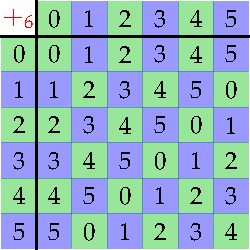
\includegraphics[scale=0.9]{factor-z6}\\
				Addition in $\Z_6$\\[5pt]
				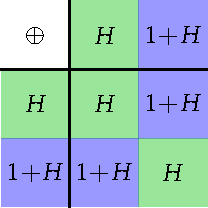
\includegraphics[scale=0.9]{factor-z6-2}\\
				Addition in $\{H,1+H\}$
			\end{tabular}
		\end{minipage}\medbreak
		To save time, we verify all possibilities simultaneously: If $x\in a+H$ and $y\in b+H$, then
		\[
			(x+y)-(a+b)=(x-a)+(y-b)\in H\implies (x+y)+H=(a+b)+H
		\]
		Addition of cosets $\oplus$ is therefore well-defined. The second table above suggests that the set of cosets forms a group under $\oplus$; indeed $\psi(x)=x+H$ defines an isomorphism of $\Z_2$ with this so-called \emph{factor group.}
	
		
% 	\exstart The set of (left) cosets for $H=\ip 4=\{0,4,8\}\le\Z_{12}$ is
% 	\[
% 		\bigl\{
% 			H,\ 1+H,\ 2+H,\ 3+H
% 		\bigr\}
% 		=\Bigl\{
% 			\{0,4,8\}, \{1,5,9\}, \{2,6,10\}, \{3,7,11\}
% 		\Bigr\}
% 	\]
% 	This feels like the cyclic group $\Z_4$ in disguise! To see this we need a binary operation: the natural approach is to use \textcolor{red}{addition} in $\Z_{12}$ to define addition of cosets via
% 	\[
% 		(a+H)\oplus(b+H):=(a\operatorname{\textcolor{red}{+}}b)+H
% 	\]
% 	This seems nice, though consider the computation more carefully:\vspace{-2pt}
% 	\begin{enumerate}\setcounter{enumi}{1}
% 	  \item[]\begin{enumeratea}
% 			\item \emph{\textbf{Choose} representatives} $a$ and $b$ in the respective cosets.
% 			\item \emph{Add within the original group} $a\operatorname{\textcolor{red}{+}}b\in\Z_{12}$.
% 			\item \emph{Take the left coset} $(a\operatorname{\textcolor{red}{+}}b)+H$.
% 		\end{enumeratea}
% 		If $\oplus$ is to make sense, the outcome $(a\operatorname{\textcolor{red}{+}}b)+H$ must be \emph{independent} of the \textbf{choices} in step (a). For instance, to properly conclude $(2+H)\oplus(3+H)=1+H$ we must check \emph{nine} possibilities
% 		\[
% 			a\in \{2,\textcolor{blue}{6},10\},\  b\in\{3,7,\textcolor{blue}{11}\} \implies a+b\in\{1,\textcolor{Green}{5},9\}
% 			\tag{one possibility is $\textcolor{blue}{6}+\textcolor{blue}{11}=\textcolor{Green}{5}\in\Z_{12}$}
% 		\]
% 		To save time, we verify all possibilities simultaneously. If $x\in a+H$ and $y\in b+H$, then
% 		\[
% 			(x+y)-(a+b)=(x-a)+(y-b)\in H\implies (x+y)+H=(a+b)+H
% 		\]
% 		Addition of cosets is therefore well-defined; indeed we'll shortly see that the set of (left) cosets forms a group under this natural addition. As you might guess, $\phi(x)=x+H$ defines an isomorphism of $\Z_4$ with this so-called \emph{factor group.}
		
	
		\item We repeat the process for the subgroup $H=\{e,\mu_1\}\le D_3$. The left cosets are
		\[
			H=\mu_1H=\{e,\mu_1\},\qquad
			\rho_1H=\mu_3H=\{\rho_1,\mu_3\},\qquad
			\rho_2H=\mu_2H=\{\rho_2,\mu_2\}
		\]
		As above, we attempt to define the `natural' operation on the set of left cosets
		\[
			aH\otimes bH:=(ab)H \tag{$ab$ is composition/multiplication within $D_3$}
		\]
		This time there is a serious problem: note that $\rho_1H=\mu_3H$, however,
		\[
			\rho_1H\otimes\rho_1H =(\rho_1\rho_1)H =\rho_2H\qquad\qquad
			\mu_3H\otimes \mu_3H=(\mu_3\mu_3)H =eH =H
		\]
		This is a contradiction: $\rho_2H\neq H$, but the result of both calculations \emph{should be the same}. The freedom of \textbf{choice} (part (a)) in the definition of $\otimes$ leads to different outcomes: the natural operation $\otimes$ \emph{does not exist} (is not well-defined), and thus cannot produce a group structure.
	\end{enumerate}
\end{examples*}



\boldsubsubsection{Well-definition of the Factor Group Structure}

The examples indicate that only some subgroups $H\le G$ behave nicely when trying to view the set of left cosets as a group. But which subgroups? To answer this question, we repeat some of our discussion abstractly. Let $H$ be a subgroup of $G$ and define the natural multiplication of left cosets\footnote{Since this operation arises naturally from that on $G$, we use the same notation (here multiplication).}
\[
	aH\cdot bH:=(ab)H \tag{$\ast$}
\]
This is well-defined precisely when
\[
	xH=aH,\ yH=bH \implies (xy)H=(ab)H \tag{$\dag$}
\]
If the natural multiplication of cosets is well-defined, the fact that $hH=H$ and $gH=gH$ for any $h\in H$, $g\in G$, tells us that
\[
 	(hg)H=gH,\text{ or equivalently }	g^{-1}hg\in H \tag{Theorem \ref{thm:cosetpart}}
\]
Since this holds \emph{for all} $g\in G$ and $h\in H$, Corollary \ref{cor:normalconj} says that \textbf{$\boldsymbol{H}$ is a normal subgroup of $\boldsymbol G$.} Not only is the converse also true, but the resulting structure forms a group under this operation.

\begin{thm}{}{}
	Suppose $H\le G$ and consider the natural operation ($\ast$) on the set of (left) cosets.
	\begin{enumerate}
	  \item ($\ast$) is well-defined if and only if $H$ is a normal subgroup of $G$.
	  \item	In such cases, $(\ast)$ defines a \emph{group structure} on the set of cosets.
	\end{enumerate}
\end{thm}

Since this process only works when $H$ is a normal subgroup, the prefix `left' is irrelevant.

\begin{defn}{}{}
	Suppose $H\triangleleft G$. The group of cosets $\quotient GH:=\bigl\{gH:g\in G\bigr\}$ \ (read '$G$ mod $H$') under the natural operation $(\ast)$ is termed a \emph{factor group} (or \emph{quotient group}).
\end{defn}

Factor group notation looks like division in part because if $G$ is finite, then $\nm{\quotient GH}=(G:H)=\frac{\nm G}{\nm H}$.

\begin{proof}
	\begin{enumerate}
	  \item\begin{description}
	  	\item[$(\Rightarrow)$] The above discussion shows that well-definition of $(\ast)$ implies $H\triangleleft G$.
	  	\item[$(\Leftarrow)$] Assume $H\triangleleft G$, and suppose $xH=aH$ and $yH=bH$. By Theorem \ref{thm:cosetpart}, $h:=x^{-1}a$ and $\tilde h:=y^{-1}b$ are both in $H$. But then,
		\[
			(xy)^{-1}(ab)=y^{-1}(x^{-1}a)b =y^{-1}hb =(y^{-1}hy)\tilde h
		\]
		which lies in $H$ by Corollary \ref{cor:normalconj} ($y^{-1}hy\in H$). We conclude that $(xy)H=(ab)H$ ($\dag$).
	  \end{description}
	  \item	Since the natural operation is well-defined, we need only verify the group axioms for $\left(\quotient GH,\cdot\right)$.
		\begin{description}
			\item[\normalfont\emph{Closure}:] Given $aH,bH\in\quotient GH$, we see that $aH\cdot bH=(ab)H$ is also coset.
			\item[\normalfont\emph{Associativity}:] $aH\cdot(bH\cdot cH)=aH\cdot(bc)H=a(bc)H$. Similarly $(aH\cdot bH)\cdot cH=(ab)cH$. By the associativity of $(G,\cdot)$, these cosets are identical.
			\item[\normalfont\emph{Identity}:] The \emph{identity coset} $H=eH$ does the job: $eH\cdot aH=(ea)H=aH=(ae)H=aH\cdot eH$.
			\item[\normalfont\emph{Inverse}:] $a^{-1}H\cdot aH=(a^{-1}a)H=eH=H$, etc., therefore $(aH)^{-1}=a^{-1}H$.\qedhere
		\end{description}
	\end{enumerate}
\end{proof}


\goodbreak


\boldsubsubsection{'Identifying' Factor Groups}

The first goal when faced with a factor group $\quotient GH$ is often to \emph{identify} it by recognizing some well-understood group to which it is isomorphic. In Section \ref{sec:1stiso} we'll develop the main piece of abstract machinery for doing this. Since this upcoming approach can be difficult to apply, it is worth first spending a little time with some basic examples. In particular, we can straightforwardly describe the factor groups of every cyclic group: by Theorem \ref{thm:cyclicisomorph}, we need only do this for $\Z$ and $\Z_n$\ldots\vspace{-5pt}



\boldinline{Factor Groups of $\Z$ (modular arithmetic done right)}

If $n$ is a positive integer, its integer multiples $n\Z=\ip n$ form a (normal) subgroup of $\Z$. The coset of $n\Z$ containing $x\in\Z$ is plainly
\[
	x+n\Z=\{x+kn:k\in\Z\}
	=\bigl\{y\in\Z:y\equiv x\negthickspace\negthickspace\pmod n\bigr\}
\]
This coset is what we have been calling `$x$' in $\Z_n$! This provides the formal definition of $\Z_n$ (superseding Definition \ref{defn:znsimple}) and trivially demonstrating that $\Z_n$ is an abelian group.

\begin{defn}{}{}
	Let $n\in\N$. The group $\Z_n$ is the factor group $\quotient{\Z}{n\Z}$.
\end{defn}

We typically drop the repeated $n\Z$ terms when calculating, recovering our familiar notation: e.g.
\[
	4+5=2\in\Z_7\quad\text{means}\quad (4+7\Z)+(5+7\Z)=2+7\Z \in\quotient{\Z}{7\Z}
\]


\boldinline{Factor Groups of Finite Cyclic Groups}

The first example on page \pageref{sec:factor} shows that $\quotient{\Z_6}{\ip 2} \cong\Z_2$. This generalizes straightforwardly.

\begin{example}{}{}
	$\ip 5=\{0,5,10,15\}\le\Z_{20}$ has factor group
	\[
		\quotient{\Z_{20}}{\ip 5}=\bigl\{\ip 5,\ 1+\ip 5,\ 2+\ip 5,\ 3+\ip 5,\ 4+\ip 5\bigr\}
	\]
	which is isomorphic to $\Z_5$ via the isomorphism
	\[
		\psi:\Z_5\to\quotient{\Z_{20}}{\ip 5}:x\mapsto x+\ip 5
	\]
\end{example}


\begin{thm}{}{znisomdefn}
	If $d\mid n$, then $\quotient{\Z_n}{\ip d}\cong\Z_d$. More generally, $\quotient{\Z_n}{\ip s}\cong\Z_{\gcd(s,n)}$.
\end{thm}

\begin{proof}
	Define $\psi:\Z_d\to\smash{\quotient{\Z_n}{\ip d}}:x\mapsto x+\ip d$. We prove that this is an isomorphism.
	\begin{description}\itemsep2pt
		\item[\normalfont\emph{Well-definition/injectivity}:] For any $x,y\in\Z_d$,
		\begin{align*}
			x=y\ (\in\Z_d)&\iff x-y\in\ip d\iff x+\ip d=y+\ip d\\
			&\iff \psi(x)=\psi(y)
		\end{align*}
		\item[\normalfont\emph{Surjectivity}:] Any coset $x+\ip d$ (being $\psi(x)$) lies in $\operatorname{range}(\psi)$.	
		\item[\normalfont\emph{Homomorphism}:] For any $x,y\in\Z_d$,
		\begin{align*}
			\psi(x+y)&=(x+y)+\ip d =\bigl(x+\ip d\bigr)+\bigl(y+\ip d\bigr)\\
			&=\psi(x)+\psi(y)
		\end{align*}
	\end{description}
	The general case follows by Corollary \ref{cor:subscyclic}: if $d=\gcd(s,n)$, then  $\ip s=\ip d$.
\end{proof}


\goodbreak


\boldinline{Further Examples}

Naïve identification of factor groups often boils down to a two-step hack.
\begin{enumerate}\itemsep2pt
  \item Find the order of the factor group $\smash{\quotient GH}$ by computing the index $(G:H)$.
  \item Determine which group of order $(G:H)$ is correct.
\end{enumerate}
If $\quotient GH$ is abelian, the Fundamental Theorem of Finitely Generated Abelian Groups (\ref{thm:fund}) might be useful for supplying candidates. Step 2 can often be accomplished by considering the possible orders of elements (cosets). With this in mind we make a minor notational observation.

\begin{lemm}{}{}
	Let $\quotient GH$ be a factor group. Then $(gH)^m=H\Longleftrightarrow g^m\in H$\quad ($mg\in H$ if $G$ additive).\par
	By Corollary \ref{cor:orderdefn}, the \textbf{order of the element} $gH\in \quotient GH$ is the smallest $m\in\N$ for which $g^m\in H$.
\end{lemm}


\begin{examples}{}{factorfiniteabelian}
	Let $G=\Z_4\times\Z_8$. We identify the factor group $\quotient GH$ for three subgroups $H$.
	\begin{enumerate}
	  \item The subgroup $H=\ip{(0,1)}=\bigl\{(0,0),(0,1),\ldots,(0,7)\bigr\}$ has 8 elements, so the factor group $\quotient GH$ has order $\frac{\nm G}{\nm H}=\frac{4\cdot 8}8=4$. By the Fundamental Theorem, $\quotient GH$ is isomorphic to $\Z_4$ or $\Z_2\times\Z_2$.\par
	  We can decide which by considering the orders of elements in $\quotient GH$:
	  \begin{quote}
	  	$\Z_2\times\Z_2$: \ Every element has order at most 2.\smallbreak
	  	$\Z_4$: \ There exists a generator with order 4.
	  \end{quote}
	  Start playing with elements (cosets)! It doesn't take long to observe that
	  \[
	  	k(1,0)=(k,0)\in H\iff 4\mid k \tag{$\dag$}
	  \]
	  Otherwise said, $(1,0)+H\in\quotient GH$ has order 4: we conclude that $\quotient GH\cong\Z_4$. Since $(1,0)+H$ is a generator, this approach provides an explicit isomorphism $\psi:\Z_4\cong\quotient GH$:
	  \[
	  	\psi(x)= (x,0)+H \hfill \Bigl(=\bigl\{ (x,0),(x,1),\ldots,(x,7)\bigr\}\!\Bigr)
		\] 	  

	  \item The subgroup $H=\ip{(0,2)}=\bigl\{(0,0),(0,2),(0,4),(0,6)\bigr\}$ has 4 elements, so $\nm{\quotient GH}=\frac{32}4=8$. The factor group is isomorphic to one of $\Z_8$, $\Z_4\times\Z_2$ or $\Z_2\times\Z_2\times\Z_2$.
	  \begin{itemize}
	    \item Exactly as in $(\dag)$, $(1,0)+H\in \quotient GH$ has order 4. This rules out $\Z_2\times\Z_2\times\Z_2$ as a candidate.
	    \item $\Z_8$ is ruled out since every $(x,y)+H$ has order at most 4: for any $(x,y)$,
	  	\[
	  		4(x,y) =(4x,4y) =(0,4y) =2y(0,2)\in H
	  	\]
	  \end{itemize}
	  By process of elimination, we conclude that $\quotient GH\cong\Z_4\times\Z_2$.

		\item\label{ex:factoriso3} The subgroup $H=\ip{(2,4)}=\bigl\{(0,0),(2,4)\bigr\}$ produces a factor group of order $\nm{\quotient GH}=\frac{32}2=16$, so we must consider \emph{five} non-isomorphic possibilities:
		\[
			\Z_{16},\quad \Z_2\times\Z_8,\quad \Z_4\times\Z_4,\quad \Z_2\times\Z_2\times\Z_4,\quad \Z_2\times\Z_2\times\Z_2\times\Z_2
		\]
		\begin{itemize}
	    \item The coset $(0,1)+H\in\quotient GH$ has order 8, since
	    \[
				k\bigl((0,1)+H\bigr)=H\iff (0,k)\in H\iff 8\mid k
			\]
			\item Every $(x,y)+H$ has order dividing 8, since
			\[
				8(x,y)=(8x,8y)=(0,0)\in H
			\]
	  \end{itemize}
	  The only candidate satisfying both properties is $\Z_2\times\Z_8$.
	\end{enumerate}
\end{examples}


\goodbreak


For factor groups of infinite or non-abelian groups, more creative strategies might be required.

\begin{examples}{}{normalmoreex}
	\exstart As seen in Exercise \ref*{sec:lagrange}.\ref{exs:index2}, every index-2 subgroup $H\le G$ is normal. Since there is only one group of order 2 up to isomorphism, in such a case $\quotient GH\cong\Z_2$.\vspace{-5pt}
	\begin{enumerate}\setcounter{enumi}{1}
	  \item[] For instance, $R_n\triangleleft D_n$ has index $(D_n:R_n)=2$. The two cosets are,\par
	  \begin{minipage}[t]{0.8\linewidth}\vspace{-18pt}
	  	\[
				\begin{array}{@{}ll}
					\text{Rotations:}&R_n=\bigl\{\rho_0,\ldots,\rho_{n-1}\bigr\}\\[3pt]
		  		\text{Reflections:}&\delta R_n=\bigl\{\delta_1,\ldots,\delta_n\bigr\}, \text{ where $\delta$ is any reflection.}
				\end{array}
		  \]
	  \end{minipage}
	  \hfill
	  \begin{minipage}[t]{0.19\linewidth}\vspace{-20pt}
	  	\flushright$\begin{array}{c||cc@{}}
	  		\circ&R_n&\delta R_n\\\hline\hline
	  		R_n&R_n&\delta R_n\\
	  		\delta R_n&\delta R_n&R_n
	  	\end{array}$
	  \end{minipage}\smallbreak
		The Cayley table for the factor group $\quotient{D_n}{R_n}=\{R_n,\delta R_n\}$ is shown. Consider how the calculation $(\delta R_n)(\delta R_n)=R_n$ says that the composition of two reflections is a rotation!
	  
% 	  \item *$\ip{2\pi}=2\pi\Z=\{2\pi n:n\in\Z\}$ is a subgroup of $(\R,+)$. In any given coset, there is a unique real number $x$ such that $0\le x<2\pi$ (think `take the remainder modulo $2\pi$'). It follows that
% 	  \[
% 	  	\quotient{\R}{2\pi\Z}=\bigl\{x+2\pi\Z:x\in[0,2\pi)\bigr\}
% 	  \]
% 	  Moreover, the function
% 	  \[
% 	  	\mu:\quotient\R{2\pi\Z}\to S^1:x+2\pi\Z\mapsto e^{ix}
% 	  \]
% 	  is a well-defined isomorphism. The factor group construction can be visualized as wrapping the real line infinitely many times around a circle of radius 1 (circumference $2\pi$).
	  
	  \item\label{ex:a4normal} In Exercise \ref*{sec:cosetnormal}.\ref{exs:va4}, we saw that the alternating group $A_4$ has the Klein four-group identified as
	  \[
			V=\bigl\{
				e,(1\,2)(3\,4),(1\,3)(2\,4),(1\,4)(2\,3)
			\bigr\}
		\]
	  as a normal subgroup. Since the factor group has order $(A_4:V)=\frac{12}4=3$ and there is only one group of order 3 up to isomorphism, we conclude that $\quotient{A_4}{V}\cong\Z_3$.%\par
		%It is harder to check, but we'll see later (Section \ref{sec:conj}) that $\quotient{S_4}{V}\cong S_3$.
	  
	  
	  \item (Example \ref*{ex:cosetexs}.\ref{ex:cosetsubspace}, simplified) \ Given $W=\{(0,y):y\in\R\}\le \R^2$, each coset (vertical line)
	  \[
	  	\bigl\{(x,y):y\in\R\bigr\}\quad \bigl(=(x,0)+W\bigr)
	  \]
	  intersects the $x$-axis at a unique point $(x,0)$. Otherwise said, we have a bijection,
	  \[
	  	\psi:\R\to\smash{\quotient{\R^2}W}:x\mapsto (x,0)+W
	  \]
	  This is moreover an isomorphism, since
	  \[
	  	\psi(x_1+x_2)=(x_1+x_2)+W= (x_1+W)+(x_2+W)=\psi(x_1)+\psi(x_2)
	  \]
	  
	  
	  \item (Hard) \ Let $G=\Z\times\Z_4$ and consider the subgroup
	  \[
	  	H=\ip{(2,1)} =\bigl\{\ldots,(-4,2),(-2,3),(0,0),(2,1),(4,2),(6,3),(8,0),(10,1),\ldots\bigr\}
	  \]
	  We cannot count cosets using the index formula. Instead we find a simple representative of each coset:
	  \[
			\begin{array}{@{}ll}
				\text{If $x=2n$ is even:}&(x,y)+H=(2n,y)+H=(0,y-n)+H\\[3pt]
	  		\text{If $x=2n+1$ is odd:}&(x,y)+H=(2n+1,y)+H=(1,y-n)+H
			\end{array}
	  \]
	  In any coset, there is a \emph{unique representative} either of the form $(0,z)$ or $(1,z)$, where $z\in\Z_4$: it follows that there are 8 cosets. To finish things off, observe that
	  \[
	  	k(1,0)=(k,0)\in H\iff 8\mid k
	  \]
		whence $(1,0)+H\in\quotient GH$ has order 8: we conclude that $\quotient GH\cong\Z_8$.
		%
% 	  \item\label{ex:hardgmodh} *Let $H=\ip{(1,2)}\le\Z\times\Z=G$. We play a similar trick to before
% 	  \[
% 	  	(x,y)+H =(0,y-2x)+(x,2x)+H =(0,y-2x)+H
% 	  \]
% 	  It follows that there is a unique representative of the form $(0,z)$ in each coset and we suspect $\quotient GH\cong\Z$. Indeed it can be verified that $\psi\bigl((x,y)+H\bigr)=y-2x$ is an isomorphism. 
	
		% 	\item\label{ex:nastyiso} Consider $H=\ip{(1,2,2)}\le G=\Z_5\times\Z_6\times\Z$. Since $G$ is infinite, we cannot simply apply the index formula to count cosets. Instead we appeal to the division algorithm.\smallbreak
		
		% 	Given $(x,y,z)$, we may subtract as many multiples of $(1,2,2)$ as we like while remaining in the same coset. It follows that each coset $(x,y,z)+H$ has a unique representative with $z=0$ or 1. In essence we are writing $z=2q+r$ where $r=0,1$ and observing that
		%   \[(x,y,z)+H=(x-q,y-2q,r)+H\]
		%   Since we have a free choice of $x\in\Z_5$ and $y\in\Z_6$ we see that there are precisely $5\cdot 6\cdot 2=60$ cosets. Since the factor group is abelian of order $60$, it must be isomorphic to one of two groups
		%   \[\Z_{60}\cong \Z_{2^2}\cdot\Z_3\times\Z_5\qquad \Z_2\times\Z_{30}\cong\Z_2\times\Z_2\times\Z_3\times\Z_5\]
		%   We distinguish between these by considering the possible orders of elements: the former requires an element of order 60. However,
		%   \[30\bigl((x,y,z)+H\bigr)=(30x,30y,30z)+H=(30x-15z,30y-30z,0)+H=H\]
		%   whence every element of the factor group $\quotient GH$ has order dividing 30.\par
		%   By elimination, we conclude that $\quotient GH\cong \Z_2\times\Z_{30}$.%\\
		%   An alternative approach, requiring a little creativity, involves spotting that
		%   \[\phi:\Z_5\times\Z_6\times\Z\mapsto\Z_5\times\Z_6\times\Z_2:(x,y,z)\mapsto (2x-z\spmod 5,y-z\spmod 6,z\spmod 2)\]
		%   is a surjective homomorphism with $\ker\phi=H$. The 1st isomorphism theorem then says that
		%   \[\mu:\quotient GH\cong \Z_5\times\Z_6\times\Z_2:(x,y,z)+H\mapsto (2x-z\spmod 5,y-z\spmod 6,z\spmod 2)\]
	\end{enumerate}
\end{examples}

We'll see more examples, and revisit other, in Section \ref{sec:1stiso} once we've developed more machinery.


\goodbreak


\begin{exercises}
	Key concepts:
	\begin{quote}
		\emph{Factor group\qquad $\quotient GH$ a group $\iff H\triangleleft G$\qquad $\Z_n:=\quotient{\Z}{n\Z}$\qquad identifying $\quotient GH$}
	\end{quote}
	
	More exs on computing say subgroup generated by a coset. Decide which problems here\ldots
	
	\begin{enumerate}
	  \item List the cosets of the subgroup $H=\ip{3}$ in $G=\Z_{15}$. By mimicking the proof of Theorem \ref{thm:znisomdefn}, show that $\psi:\Z_3\mapsto \quotient GH:x\mapsto x+H$ is a well-defined homomorphism.
% 	  \[
% 	  	\psi:\Z_3\mapsto \quotient GH:x\mapsto x+H
% 	  \]
	
		
		\item  (Recall Exercise \ref*{sec:cosetnormal}.\ref{exs:VfactorV})\lstsp If $H=\bigl\{(0,0),(0,2),(2,0),(2,2)\bigr\}$, identify the factor group $\quotient{\Z_4\times\Z_4}H$.
		
		
		\item Identify the factor group $\quotient GH$ where $H=\ip{(2,4)}\le G=\Z_4\times\Z_6$.
		  %\item Repeat with the subgroup $H=\ip 2\times\ip 4$ (\emph{this is a trick question!})
		
		
		\item\begin{enumerate}
		  \item Let $G=\Z_9\times\Z_9$ and $H=\ip{(3,6)}$. Identify $\quotient GH$ by showing that every element of the factor group has order at most 9 and that it contains an element of order 9.
		  
		  \item Repeat with $H=\ip 3\times\ip 6$ \ (\emph{this \textbf{isn't} a trick question}).
		\end{enumerate}
	  
	  
		\item Let $G$ be any group. To what groups are $\quotient G{\{e\}}$ and $\quotient GG$ isomorphic?
		
	
		\item\label{exs:gmodhabelian}\begin{enumerate}
		  \item If $G$ is abelian and $H\le G$, prove that $\quotient GH$ is abelian.
		  
		  \item If $\quotient GH$ is abelian, can we conclude that $G$ and/or $H$ is abelian? Explain.
		\end{enumerate}
		
	
	 	\item* HARD (See Examples \ref{ex:factorfiniteabelian})\lstsp Let $G=\Z_4\times\Z_8$. Prove that each $\psi$ is a well-defined homomorphism:
		\begin{enumerate}\itemsep0pt
			\item $H=\ip{(0,1)}$, \ $\psi:\Z_4\to\quotient GH:x\mapsto (x,0)+H$
			\item $H=\ip{(0,2)}$, \ $\psi:\Z_4\times\Z_2\to\quotient GH:(x,y)\mapsto (x,y)+H$
			\item $H=\ip{(2,4)}$, \ $\psi:\Z_2\times\Z_8\to\quotient GH:(x,y)\mapsto (x,y-2x)+H$
		\end{enumerate}
		(\emph{Bijectivity follows from the description of the cosets, though proving injectivity might be instructive.})
		
		
		\item Revisit Exercise \ref*{sec:lagrange}.\ref{exs:zsqrt2subgroup}. The factor group $\quotient GH$ is abelian and of order 6, whence it is cyclic. Prove this explicitly by finding a generator and thus an isomorphism $\psi:\Z_6\to\quotient GH$.
		
		
		\item\begin{enumerate}
	  	\item Let $G$ be a cyclic group with subgroup $H$. Prove that $\quotient GH$ is cyclic.
	  	\item If $\quotient GH$ is cyclic, does it follow that $G$ is cyclic? Explain.
		\end{enumerate}
	
	
		\item In Example \ref*{ex:normalmoreex}.\ref{ex:a4normal} we saw that $\Z_3\cong\quotient{A_4}{V}$. Find an explicit isomorphism.
			
	
		\item Exercise \ref*{sec:cosetnormal}.\ref{exs:d4normal} showed that $\{\rho_0,\rho_2\}$ is a normal subgroup of $D_4$. To what well-known group is the factor group $\quotient{D_4}{\{\rho_0,\rho_2\}}$ isomorphic? Prove your assertion.
		
	
		\item\begin{enumerate}
		  \item Identify the factor group $\quotient{S_n}{A_n}\cong K$ where $K$ is some well-understood basic group. Describe an explicit isomorphism $\psi:K\to\quotient{S_n}{A_n}$ and verify that it is such.
		  \item Repeat for the factor group $\quotient{\rO_n(\R)}{\rSO_n(\R)}$.
		\end{enumerate}
		
		
		\item\label{exs:normaldirectfactor} (Recall Exercise \ref*{sec:cosetnormal}.\ref{exs:directprodfactor})\lstsp Suppose $G=H\times K$, $J\triangleleft H$ and $\widehat J=J\times\{e_K\}$. Prove that $\quotient G{\widetilde J}=\quotient HJ\times K$.\par
		Can you quickly verify Examples \ref{ex:factorfiniteabelian}.1, 2, and \ref{ex:normalmoreex}.1 in this language?
		
		
		\item (Hard) \ Let $H=\ip{(2,3)}\le G=\Z_5\times \Z$. Prove that $\quotient GH\cong \Z_{15}$.
		
		
		\item* Verify the claim in Example \ref*{ex:normalmoreex}.\ref{ex:hardgmodh} that $\psi\bigl((x,y)+H\bigr)=y-2x$ is an isomorphism.
		
		
		\item (Hard!) \ If $G=\Z_{10}\times\Z_6\times\Z$ and $H=\ip{(4,2,3)}$, identify $\quotient GH$ as a direct product $\Z_m\times\Z_n$.\par
		(\emph{Hint: show that exactly one representative of the coset $(x,y,z)+H$ has $z= 0, 1$ or 2})
		
		
		%   \item Let $G=\Z_{10}\times\Z_6\times\Z$ and $H=\ip{(4,2,3)}$. Since the groups are infinite, we cannot use the index formula to count cosets.
	%   We sketch the process for identifying $\quotient GH$: the details of parts (b), (c) and (d) are an exercise with some hints.
	%   \begin{enumerate}
	%     \item Apply the division algorithm: $z=3q+r$ where $r=0,1,2$ and observe that
	%   	\[(x,y,z)+H=(x,y,z)-q(4,2,3)+H=(x-4q,y-2q,r)+H\]
	%   	Every coset therefore contains precisely one element $(x,y,z)$ where either $z=0,1$ or 2.
	%   	\item The elements $(x,y,0),(x,y,1)$ and $(x,y,2)$ where $x\in\Z_{10}$ and $y\in\Z_6$ are shown to lie in different cosets. There are therefore $180=2^2\cdot 3^2\cdot 5$ cosets which yield four non-isomorphic possibilities for the factor group:
	%   	\[\Z_{180},\ \ \Z_2\times\Z_{90},\ \ \Z_3\times\Z_{60},\ \ \Z_6\times\Z_{30}\]
	%   	\item The coset $(1,1,1)+H$ has order 90.
	% %   	\[n(1,1,1)\in H\implies n=3k\implies (n-2k,n-4k,0)\in H\]
	% %   	\begin{align*}
	% %   		3k(1,1,1)+H&=(3k,3k,3k)+H=(3k,3k,3k)-k(4,2,3)+H\tag*{(since $(4,2,3)\in H$)}\\
	% %   		&=(-k,k,0)+H\\
	% %   		&=H\iff 10\mid k\ \text{and}\ 6\mid k \iff 30\mid k\iff 90\mid n
	% %   	\end{align*}
	%   	\item Every coset $(x,y,z)+H$ has order dividing 90.
	%   \end{enumerate}
	%   We conclude that $\quotient GH\cong \Z_2\times\Z_{90}$.
	
	% 	\begin{itemize}
	%   \item : if two such were in the same coset, then
	%   \begin{align*}
	%   (x_1,y_1,0)-(x_2,y_2,0)\in H&\iff (x_1-x_2,y_1-y_2,0)\in H\\
	%   &\iff\begin{cases}
	%   x_1\equiv x_2\pmod{10}\\
	%   \qquad\quad\text{and}\\
	%   y_1\equiv y_2\pmod{6}
	%   \end{cases}
	%   \end{align*}
	%   Similarly all the elements $(x,y,1)$ and $(x,y,2)$ lie in different cosets.
	%   \item It follows that the elements $(x,y,0)$, $(x,y,1)$ and $(x,y,2)$ are representatives of different cosets, and that all cosets have one such representative. There are therefore $10\cdot 6\cdot 3=180$ distinct cosets whence the factor group $\quotient GH$ is abelian of order 180.
	%   \item The prime decomposition of $180$ is $2^2\cdot 3^2\cdot 5$: there are, up to isomorphism, \emph{four} abelian groups of order 180, namely
	%   \begin{gather*}
	%   \Z_4\times\Z_9\times\Z_5\cong\Z_{180}\\
	%   \Z_2\times\Z_2\times\Z_9\times\Z_5\cong\Z_2\times\Z_{90}\\
	%   \Z_4\times\Z_3\times\Z_3\times\Z_5\cong\Z_3\times\Z_{60}\\
	%   \Z_2\times\Z_2\times\Z_3\times\Z_3\times\Z_5\cong\Z_6\times\Z_{30}
	%   \end{gather*}
	%   How do we distinguish between these? As before, we look for elements of a particular order (lots of scratch work may be required in general!).
	%   \item Compute the order of the coset $(1,1,1)+H$. Certainly its order must be divisible by 3, since the third entry of
	%   \[n(1,1,1)=(n,n,n)\in H\]
	%   requires $3\mid n$. Thus let $n=3k$. Now
	%   \begin{align*}
	%   3k(1,1,1)+H&=(3k,3k,3k)+H=(3k,3k,3k)-k(4,2,3)+H\tag*{(since $(4,2,3)\in H$)}\\
	%   &=(-k,k,0)+H\\
	%   &=H\iff 10\mid k\ \text{and}\ 6\mid k \iff 30\mid k\iff 90\mid n
	%   \end{align*}
	%   Since $\quotient GH$ contains an element of order 90, our choices are narrowed to $\Z_{180}$ and $\Z_2\times\Z_{90}$.
	%   \item We show that \emph{every} element of $\quotient GH$ has order dividing 90:
	%   \begin{align*}
	%   90\bigl((x,y,z)+H\bigr)&=(90x,90y,90z)-30z(4,2,3)+H=(90x-120z,90y-60z,0)+H\\
	%   &=(0,0,0)+H
	%   \end{align*}
	%   We conclude that $\quotient GH\cong\Z_2\times\Z_{90}$. Phew!
	% \end{itemize}
	% You can check (it's hard!) that the function
	% \[\psi:\Z_2\times\Z_{90}\to\quotient{(\Z_{10}\times\Z_6\times\Z)}{\ip{(4,2,3)}}:(x,y)\mapsto(y,3x+y,y)+H\]
	% is an isomorphism, though you'd have to be truly inspired to conjecture this out of thin air!
		
		
	\end{enumerate}

\end{exercises}



